\documentclass{beamer}

\title[CSE 300 Technical Writing and Presentation]{Safe Labeling of Graphs with Minimum Span}
\author[1605042 \& 1605038]{Authors:\\Md. Saidur Rahman , Umma Habiba\\Shah Hasnat Lamia, Tahmima Chowdhury\\~\\Presented By:\\1605038 \quad \& \quad 1605042}
\institute[]{Department of Computer Science and Engineering \linebreak
	Bangladesh University of Engineering and Technology\linebreak
	\includegraphics[height=1.5cm,width=1.5cm]{buetlogo.png}}
\date{September 7, 2019}

\usepackage{verbatim}
\usepackage{tikz}
\usetikzlibrary{shadings, patterns, shapes.geometric}
\usepackage{graphicx}
\usepackage{subcaption}
\usepackage{amsmath}
\usepackage{mwe}
\usetheme{Madrid}
\usepackage{xcolor}

\definecolor{beaublue}{rgb}{0.74, 0.83, 0.9}
\definecolor{ao(english)}{rgb}{0.0, 0.5, 0.0}
\definecolor{calpolypomonagreen}{rgb}{0.12, 0.3, 0.17}
\definecolor{amethyst}{rgb}{0.6, 0.4, 0.8}
\definecolor{candyapplered}{rgb}{1.0, 0.03, 0.0}
\setbeamertemplate{frametitle}[default][center]
\begin{document}
	
\begin{frame}
\titlepage
\end{frame}

	\section{Introduction to Safe labeling and Minimum Span}
		\begin{frame}
			\frametitle{Outline}
			\tableofcontents[currentsection]
		\end{frame}
	\begin{frame}{\textit{k}-safe Labeling of Graph}
		\begin{center}
		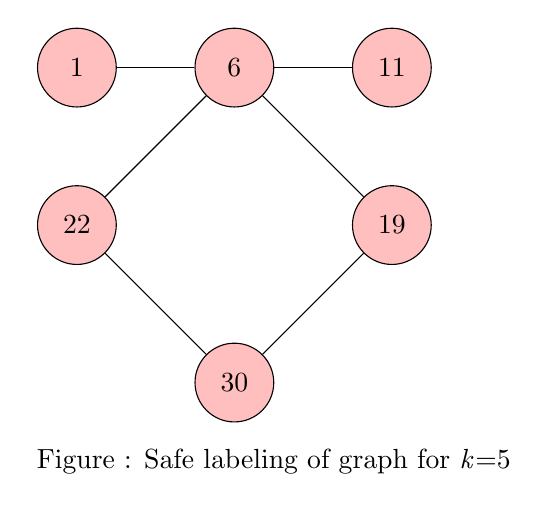
\begin{tikzpicture}
		\tikzstyle{vertex} = [circle,fill=pink,draw=black]
		\tikzstyle{edge} = [-]
		\node[vertex,minimum size=1cm] (n1) at (0,0) {1};
		\node[vertex,minimum size=1cm] (n2) at (2,0) {6};
		\node[vertex,minimum size=1cm] (n3) at (4,0) {11};
		\node[vertex,minimum size=1cm] (n4) at (0,-2) {22};
		\node[vertex,minimum size=1cm] (n5) at (4,-2) {19};
		\node[vertex,minimum size=1cm] (n6) at (2,-4) {30};
		\draw[edge] (n1)--(n2);
		\draw[edge] (n3)--(n2);
		\draw[edge] (n2)--(n4);
		\draw[edge] (n5)--(n2);
		\draw[edge] (n6)--(n4);
		\draw[edge] (n5)--(n6);
		\node[] (n7) at (2.5,-5) {Figure : Safe labeling of graph for \textit{k}=5};
		\end{tikzpicture}	
	\end{center}
	\begin{itemize}
		\item<2-> Span of $k$-safe labeling = $I_l - I_s +1$
			\item<3-> For this graph , Span = $30-1+1=30$
	\end{itemize}
	
	\end{frame}
	
		\begin{frame}{Minimum Span}
			\begin{columns}
				\column{0.45\textwidth}
					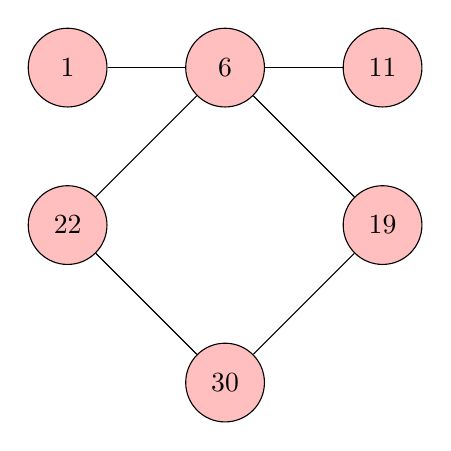
\begin{tikzpicture}
					\tikzstyle{vertex} = [circle,fill=pink,draw=black]
					\tikzstyle{edge} = [-]
					\node[vertex,minimum size=1cm] (n1) at (0,0) {1};
					\node[vertex,minimum size=1cm] (n2) at (2,0) {6};
					\node[vertex,minimum size=1cm] (n3) at (4,0) {11};
					\node[vertex,minimum size=1cm] (n4) at (0,-2) {22};
					\node[vertex,minimum size=1cm] (n5) at (4,-2) {19};
					\node[vertex,minimum size=1cm] (n6) at (2,-4) {30};
					\draw[edge] (n1)--(n2);
					\draw[edge] (n3)--(n2);
					\draw[edge] (n2)--(n4);
					\draw[edge] (n5)--(n2);
					\draw[edge] (n6)--(n4);
					\draw[edge] (n5)--(n6);
					\end{tikzpicture}
					\begin{center}
						\textbf{Span = 30}
					\end{center}
				
				\column{0.1\textwidth}
				\includegraphics[width=1.2cm,height=1cm]{arrow.png}
				\column{0.45\textwidth}
					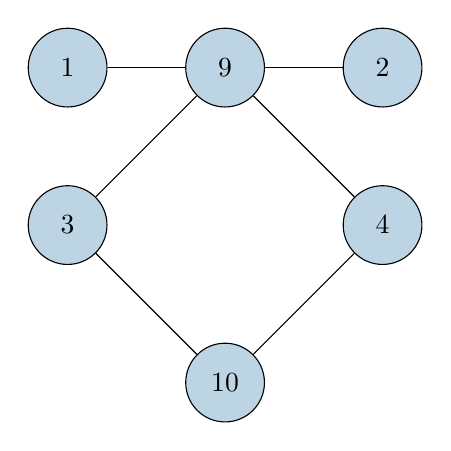
\begin{tikzpicture}
					\tikzstyle{vertex} = [circle,fill=beaublue,draw=black,radius=25pt]
					\tikzstyle{edge} = [-]
					\node[vertex,minimum size=1cm] (n1) at (7,0) {1};
					\node[vertex,minimum size=1cm] (n2) at (9,0) {9};
					\node[vertex,minimum size=1cm] (n3) at (11,0) {2};
					\node[vertex,minimum size=1cm] (n4) at (7,-2) {3};
					\node[vertex,minimum size=1cm] (n5) at (11,-2) {4};
					\node[vertex,minimum size=1cm] (n6) at (9,-4) {10};
					\draw[edge] (n1)--(n2);
					\draw[edge] (n3)--(n2);
					\draw[edge] (n2)--(n4);
					\draw[edge] (n5)--(n2);
					\draw[edge] (n6)--(n4);
					\draw[edge] (n5)--(n6);
					\end{tikzpicture}
					\begin{center}
						\textbf{Span = 10}
						
						(Minimum Span)
					\end{center}
			\end{columns}
			
			
		\end{frame}
		
	\begin{frame}{\textit{k}-safe Labeling Problem}
	\begin{block}{Problem Statement}
	The \textit{k-safe labeling problem} asks to find a $k$-safe labeling of a graph with minimum span
	\end{block}
		
	\end{frame}
	
		\begin{frame}{What is Antibandwidth problem ? }
			\begin{center}
				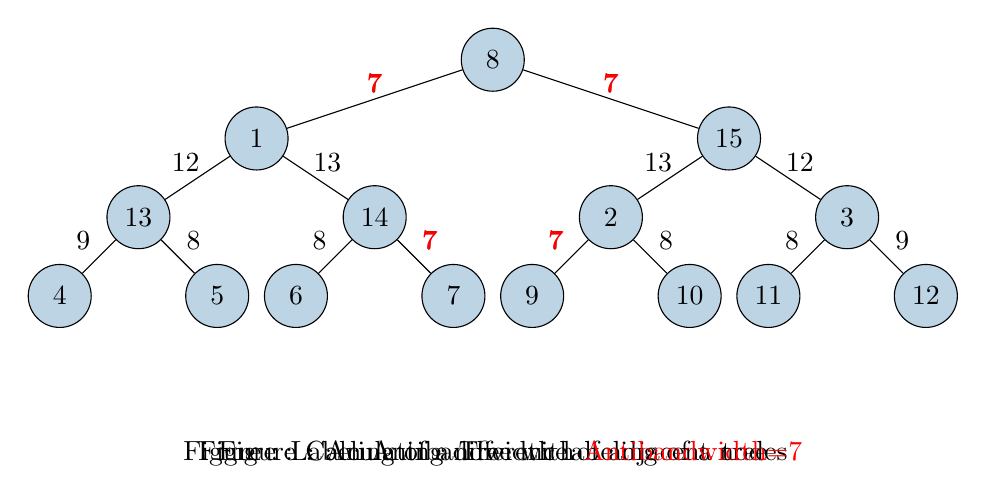
\begin{tikzpicture}
				\tikzstyle{vertex} = [circle,fill=beaublue,draw=black]
				\tikzstyle{edge} = [-]
				\node[vertex,minimum size=0.8cm] (n1) at (0,0) {8};
				\node[vertex,minimum size=0.8cm] (n2) at (-3,-1) {1};
				\node[vertex,minimum size=0.8cm] (n3) at (3,-1) {15};
				\node[vertex,minimum size=0.8cm] (n4) at (-4.5,-2) {13};
				\node[vertex,minimum size=0.8cm] (n5) at (-1.5,-2) {14};
				\node[vertex,minimum size=0.8cm] (n6) at (4.5,-2) {3};
				\node[vertex,minimum size=0.8cm] (n7) at (1.5,-2) {2};
				\node[vertex,minimum size=0.8cm] (n8) at (-5.5,-3) {4};
				\node[vertex,minimum size=0.8cm] (n9) at (-3.5,-3) {5};
				\node[vertex,minimum size=0.8cm] (n10) at (-0.5,-3) {7};
				\node[vertex,minimum size=0.8cm] (n11) at (-2.5,-3) {6};
				\node[vertex,minimum size=0.8cm] (n12) at (0.5,-3) {9};
				\node[vertex,minimum size=0.8cm] (n13) at (2.5,-3) {10};
				\node[vertex,minimum size=0.8cm] (n14) at (3.5,-3) {11};
				\node[vertex,minimum size=0.8cm] (n15) at (5.5,-3) {12};
				\draw[edge] (n1)--(n2);
				\draw[edge] (n1)--(n3);
				\draw[edge] (n2)--(n4);
				\draw[edge] (n2)--(n5);
				\draw[edge] (n3)--(n6);
				\draw[edge] (n3)--(n7);
				\draw[edge] (n4)--(n8);
				\draw[edge] (n4)--(n9);
				\draw[edge] (n5)--(n10);
				\draw[edge] (n5)--(n11);
				\draw[edge] (n7)--(n12);
				\draw[edge] (n7)--(n13);
				\draw[edge] (n6)--(n14);
				\draw[edge] (n6)--(n15);
				
				\node<1-1>[] (n20) at (0,-5) {Figure : An Antibandwidth labeling of a tree  };
				\node<2-2>[] (s1) at (-1.5,-0.3) {\textcolor{black}{7}};
				\node<2-2>[] (s4) at (1.5,-0.3) {\textcolor{black}{7}};
				\node<2->[] (s2) at (-3.9,-1.3) {\textcolor{black}{12}};
				\node<2->[] (s3) at (3.9,-1.3) {\textcolor{black}{12}};
				\node<2->[] (s5) at (-2.1,-1.3) {\textcolor{black}{13}};
				\node<2->[] (s6) at (2.1,-1.3) {\textcolor{black}{13}};
				\node<2->[] (s7) at (-5.2,-2.3) {\textcolor{black}{9}};
				\node<2->[] (s8) at (-3.8,-2.3) {\textcolor{black}{8}};
				\node<2->[] (s9) at (5.2,-2.3) {\textcolor{black}{9}};
				\node<2->[] (s10) at (3.8,-2.3) {\textcolor{black}{8}};
				\node<2->[] (s11) at (-2.2,-2.3) {\textcolor{black}{8}};
				\node<2-2>[] (s12) at (-0.8,-2.3) {\textcolor{black}{7}};
				\node<2->[] (s13) at (2.2,-2.3) {\textcolor{black}{8}};
				\node<2-2>[] (s14) at (0.8,-2.3) {\textcolor{black}{7}};
				\node<2-2>[] (n20) at (0,-5) {Figure : Calculating difference of adjacent nodes};
				\node<3->[] (r1) at (-1.5,-0.3) {\textcolor{red}{\textbf{7}}};
				\node<3->[] (r4) at (1.5,-0.3) {\textcolor{red}{\textbf{7}}};
				\node<3->[] (r12) at (-0.8,-2.3) {\textcolor{red}{\textbf{7}}};
				\node<3->[] (r14) at (0.8,-2.3) {\textcolor{red}{\textbf{7}}};
				\node<3->[] (n20) at (0,-5) {Figure : Labeling of a Tree with \textcolor{red}{Antibandwidth=7}};
				\end{tikzpicture}	
			\end{center}	
			
		\end{frame}
		\begin{frame}{Motivation}
			\centering
			\includegraphics[width=9cm,height=6cm]{towers.jpg}
			
		\end{frame}
	
	\section{Hardness of Safe Labeling Problem}
		\begin{frame}
			\frametitle{Outline}
			\tableofcontents[currentsection]
		\end{frame}
		
	\begin{frame}{Hardness of Safe Labeling Problem}
		\begin{block}{\textit{k}-safe labeling problem is NP-Hard }
			We can reduce the Antibandwidth problem to \textit{k}-safe labeling problem and thus successfully prove that \textit{k}-safe labeling problem is NP-Hard.
		\end{block}
		\textcolor{white}{a couple of words}\linebreak
		\textcolor{white}{a couple of words}\linebreak
		\uncover<2->{\includegraphics[width=12cm,height=2.5cm]{blackbox.png}}
		
	\end{frame}
	
	\begin{frame}{Decision version of Antibandwidth problem}
			\begin{tikzpicture}
			\tikzstyle{vertex} = [circle,fill=beaublue,draw=black]
			\tikzstyle{edge} = [-]
			\node[vertex,minimum size=0.8cm] (n1) at (0,0) {8};
			\node[vertex,minimum size=0.8cm] (n2) at (-3,-1) {1};
			\node[vertex,minimum size=0.8cm] (n3) at (3,-1) {15};
			\node[vertex,minimum size=0.8cm] (n4) at (-4.5,-2) {13};
			\node[vertex,minimum size=0.8cm] (n5) at (-1.5,-2) {14};
			\node[vertex,minimum size=0.8cm] (n6) at (4.5,-2) {3};
			\node[vertex,minimum size=0.8cm] (n7) at (1.5,-2) {2};
			\node[vertex,minimum size=0.8cm] (n8) at (-5.5,-3) {4};
			\node[vertex,minimum size=0.8cm] (n9) at (-3.5,-3) {5};
			\node[vertex,minimum size=0.8cm] (n10) at (-0.5,-3) {7};
			\node[vertex,minimum size=0.8cm] (n11) at (-2.5,-3) {6};
			\node[vertex,minimum size=0.8cm] (n12) at (0.5,-3) {9};
			\node[vertex,minimum size=0.8cm] (n13) at (2.5,-3) {10};
			\node[vertex,minimum size=0.8cm] (n14) at (3.5,-3) {11};
			\node[vertex,minimum size=0.8cm] (n15) at (5.5,-3) {12};
			\draw[edge] (n1)--(n2);
			\draw[edge] (n1)--(n3);
			\draw[edge] (n2)--(n4);
			\draw[edge] (n2)--(n5);
			\draw[edge] (n3)--(n6);
			\draw[edge] (n3)--(n7);
			\draw[edge] (n4)--(n8);
			\draw[edge] (n4)--(n9);
			\draw[edge] (n5)--(n10);
			\draw[edge] (n5)--(n11);
			\draw[edge] (n7)--(n12);
			\draw[edge] (n7)--(n13);
			\draw[edge] (n6)--(n14);
			\draw[edge] (n6)--(n15);
			
			\node<2-> (img) at (4.5,1) {\includegraphics[width=2cm,height=2cm]{qus.png}};
			\end{tikzpicture}	
				\textcolor{white}{a couple of words}	
		\begin{itemize}
			\item<1->[$\bigstar$] An Antibandwidth labeling with \textit{\textcolor{ao(english)}{n = 15}} and \textit{\textcolor{ao(english)}{k = 7}};
			\item<2-2>[]\textcolor{red}{ But how can we reduce this to \textit{k}-safe labeling problem?}
		\end{itemize}
		
	\end{frame}
		\begin{frame}{Reduction to \textit{k}-safe Labeling Problem}
			\begin{tikzpicture}
			\tikzstyle{vertex} = [circle,fill=beaublue,draw=black]
			\tikzstyle{edge} = [-]
			\node[vertex,minimum size=0.8cm] (n1) at (0,0) {8};
			\node[vertex,minimum size=0.8cm] (n2) at (-3,-1) {1};
			\node[vertex,minimum size=0.8cm] (n3) at (3,-1) {15};
			\node[vertex,minimum size=0.8cm] (n4) at (-4.5,-2) {13};
			\node[vertex,minimum size=0.8cm] (n5) at (-1.5,-2) {14};
			\node[vertex,minimum size=0.8cm] (n6) at (4.5,-2) {3};
			\node[vertex,minimum size=0.8cm] (n7) at (1.5,-2) {2};
			\node[vertex,minimum size=0.8cm] (n8) at (-5.5,-3) {4};
			\node[vertex,minimum size=0.8cm] (n9) at (-3.5,-3) {5};
			\node[vertex,minimum size=0.8cm] (n10) at (-0.5,-3) {7};
			\node[vertex,minimum size=0.8cm] (n11) at (-2.5,-3) {6};
			\node[vertex,minimum size=0.8cm] (n12) at (0.5,-3) {9};
			\node[vertex,minimum size=0.8cm] (n13) at (2.5,-3) {10};
			\node[vertex,minimum size=0.8cm] (n14) at (3.5,-3) {11};
			\node[vertex,minimum size=0.8cm] (n15) at (5.5,-3) {12};
			\draw[edge] (n1)--(n2);
			\draw[edge] (n1)--(n3);
			\draw[edge] (n2)--(n4);
			\draw[edge] (n2)--(n5);
			\draw[edge] (n3)--(n6);
			\draw[edge] (n3)--(n7);
			\draw[edge] (n4)--(n8);
			\draw[edge] (n4)--(n9);
			\draw[edge] (n5)--(n10);
			\draw[edge] (n5)--(n11);
			\draw[edge] (n7)--(n12);
			\draw[edge] (n7)--(n13);
			\draw[edge] (n6)--(n14);
			\draw[edge] (n6)--(n15);
			
			\node (img) at (4.5,1) {\includegraphics[width=2cm,height=2cm]{idea.png}};
			\end{tikzpicture}	
			\textcolor{white}{a couple of words}	
			\begin{itemize}
				\item[$\bigstar$] An Antibandwidth labeling with \textit{\textcolor{ao(english)}{n = 15}} and \textit{\textcolor{ao(english)}{k = 7}};
				\item[\textcolor{calpolypomonagreen}{$\checkmark$}]\textcolor{calpolypomonagreen}{If we set \textit{s = n =15} and \textit{k = 7} }
			\end{itemize}
			
		\end{frame}
		\section{k-safe Labeling of Bipartite  Graphs}
		\begin{frame}
			\frametitle{Outline}
			\tableofcontents[currentsection]
		\end{frame}
		\begin{frame}{What is Bipartiate Graph?}
			\centering
			\includegraphics[height=5cm,width=8cm]{nocolor.png}
			\\~\\
			Figure:A Bipartite Graph
		\end{frame}
		\begin{frame}{Two coloring of a Bipartiate Graph}
			\centering
			\includegraphics[height=5cm,width=8cm]{twocolor.png}
			\\~\\
			Figure:A Bipartite Graph is a Two-Coloring Graph
		\end{frame}
			\begin{frame}{Upper Bound on the Span of Bipartite Graphs }
				\begin{block}{\textit{k}-safe labeling of Bipartite Graphs }
					A Bipartite Graph of \textit{n} vertices admits a \textit{k}-safe labeling of
					\textit{n+k-1} , and such a
					labeling can be computed in linear time.
				\end{block}
				\textcolor{white}{a couple of words} \linebreak
				\centering
				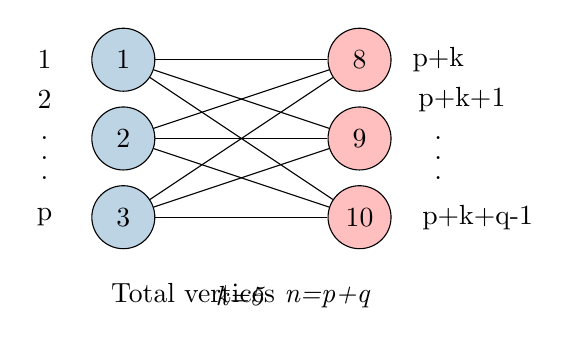
\begin{tikzpicture}
				\tikzstyle{vertex} = [circle,fill=beaublue,draw=black]
				\tikzstyle{vertex2} = [circle,fill=pink,draw=black]
				\tikzstyle{edge} = [-]
				\node<1->[vertex,minimum size=0.8cm] (n1) at (0,0) {};
				\node<1->[vertex,minimum size=0.8cm] (n2) at (0,-1) {};
				\node<1->[vertex,minimum size=0.8cm] (n3) at (0,-2) {};
				\node<1->[vertex2,minimum size=0.8cm] (n4) at (3,0) {};
				\node<1->[vertex2,minimum size=0.8cm] (n5) at (3,-1) {};
				\node<1->[vertex2,minimum size=0.8cm] (n6) at (3,-2) {};
				\node<2->[] (p1) at (-1,0) {1};
				\node<2->[] (p2) at (-1,-0.5) {2};
				\node<2->[] (p3) at (-1,-1) {.};
				\node<2->[] (p6) at (-1,-1.25) {.};
				\node<2->[] (p4) at (-1,-1.5) {.};
				\node<2->[] (p5) at (-1,-2) {p};
				
				\node<3->[] (p1) at (4,0) {p+k};
				\node<3->[] (p2) at (4.3,-0.5) {p+k+1};
				\node<3->[] (p3) at (4,-1) {.};
				\node<3->[] (p6) at (4,-1.25) {.};
				\node<3->[] (p4) at (4,-1.5) {.};
				\node<3->[] (p5) at (4.5,-2) {p+k+q-1};
				\draw[edge] (n1)--(n4);
				\draw[edge] (n1)--(n5);
				\draw[edge] (n1)--(n6);
				\draw[edge] (n2)--(n4);
				\draw[edge] (n2)--(n5);
				\draw[edge] (n2)--(n6);
				\draw[edge] (n3)--(n4);
				\draw[edge] (n3)--(n5);
				\draw[edge] (n3)--(n6);
				\node<2-3>[] (f1) at (1.5,-3) {Total vertices \textit{n=p+q}};
				
				\node<4->[] (l1) at (0,0) {1};
				\node<5->[] (l2) at (0,-1) {2};
				\node<6->[] (l3) at (0,-2) {3};
				\node<7->[] (l4) at (3,0) {8};
				\node<8->[] (l5) at (3,-1) {9};
				\node<9->[] (l6) at (3,-2) {10};
				
				\node<7-9>[] (f2) at (1.5,-3) {\textit{k=5}};
				\end{tikzpicture}
				\begin{itemize}
					\item<10-> Minimum distance of labels of two adjacent vertices is at least \textit{p+k-p=k}
					\item<11-> Span = \textit{p+k+q-1=n+k-1}
				\end{itemize}
			\end{frame}
			
				\section{k-safe Labeling of Trees}
				\begin{frame}
					\frametitle{Outline}
					\tableofcontents[currentsection]
				\end{frame}
				\begin{frame}{Upper Bound on the Span of Trees }
					\begin{block}{\textit{k}-safe labeling of Trees }
						Every Tree with \textit{n} vertices admits a \textit{k}-safe labeling of
						\textit{n+k-1} , and such a
						labeling can be computed in linear time.
					\end{block}
					\begin{center}
						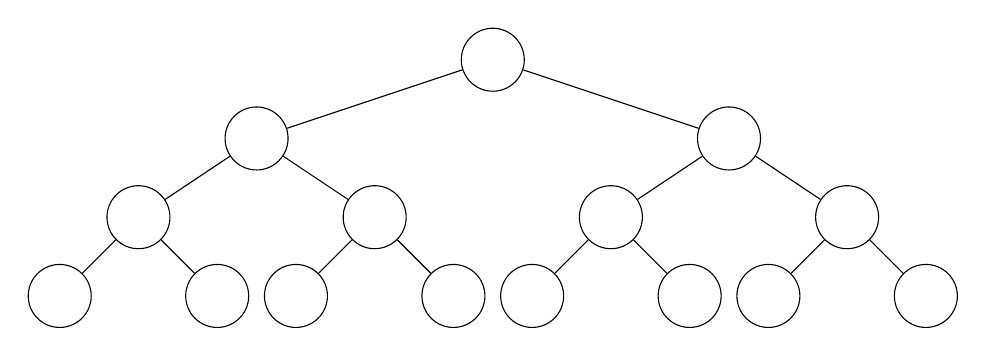
\begin{tikzpicture}
						\tikzstyle{vertex} = [circle,fill=white,draw=black]
						\tikzstyle{vertex2} = [circle,fill=white,draw=black]
						\tikzstyle{edge} = [-]
						\node[vertex,minimum size=0.8cm] (n1) at (0,0) {};
						\node[vertex2,minimum size=0.8cm] (n2) at (-3,-1) {};
						\node[vertex2,minimum size=0.8cm] (n3) at (3,-1) {};
						\node[vertex,minimum size=0.8cm] (n4) at (-4.5,-2) {};
						\node[vertex,minimum size=0.8cm] (n5) at (-1.5,-2) {};
						\node[vertex,minimum size=0.8cm] (n6) at (4.5,-2) {};
						\node[vertex,minimum size=0.8cm] (n7) at (1.5,-2) {};
						\node[vertex2,minimum size=0.8cm] (n8) at (-5.5,-3) {};
						\node[vertex2,minimum size=0.8cm] (n9) at (-3.5,-3) {};
						\node[vertex2,minimum size=0.8cm] (n10) at (-0.5,-3) {};
						\node[vertex2,minimum size=0.8cm] (n11) at (-2.5,-3) {};
						\node[vertex2,minimum size=0.8cm] (n12) at (0.5,-3) {};
						\node[vertex2,minimum size=0.8cm] (n13) at (2.5,-3) {};
						\node[vertex2,minimum size=0.8cm] (n14) at (3.5,-3) {};
						\node[vertex2,minimum size=0.8cm] (n15) at (5.5,-3) {};
						\draw[edge] (n1)--(n2);
						\draw[edge] (n1)--(n3);
						\draw[edge] (n2)--(n4);
						\draw[edge] (n2)--(n5);
						\draw[edge] (n3)--(n6);
						\draw[edge] (n3)--(n7);
						\draw[edge] (n4)--(n8);
						\draw[edge] (n4)--(n9);
						\draw[edge] (n5)--(n10);
						\draw[edge] (n5)--(n11);
						\draw[edge] (n7)--(n12);
						\draw[edge] (n7)--(n13);
						\draw[edge] (n6)--(n14);
						\draw[edge] (n6)--(n15);
						\end{tikzpicture}	
					\end{center}	
					
				\end{frame}
			\begin{frame}{Upper Bound on the Span of Trees }
				\begin{block}{\textit{k}-safe labeling of Trees }
					Every Tree with \textit{n} vertices admits a \textit{k}-safe labeling of
					\textit{n+k-1} , and such a
					labeling can be computed in linear time.
				\end{block}
				\begin{center}
					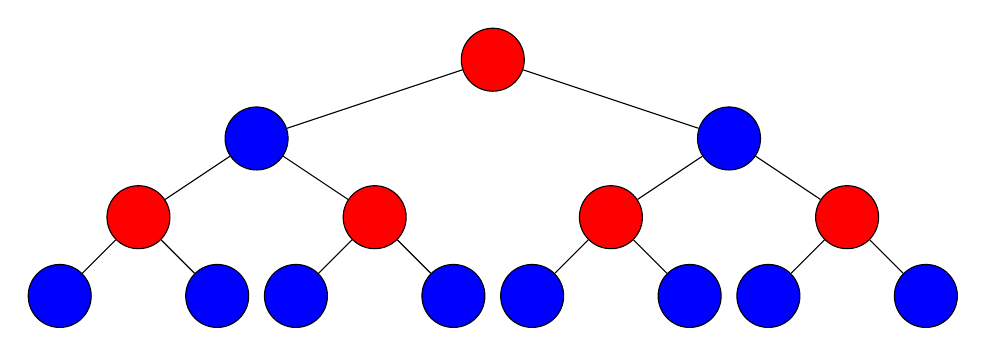
\begin{tikzpicture}
					\tikzstyle{vertex} = [circle,fill=red,draw=black]
					\tikzstyle{vertex2} = [circle,fill=blue,draw=black]
					\tikzstyle{edge} = [-]
					\node[vertex,minimum size=0.8cm] (n1) at (0,0) {};
					\node[vertex2,minimum size=0.8cm] (n2) at (-3,-1) {};
					\node[vertex2,minimum size=0.8cm] (n3) at (3,-1) {};
					\node[vertex,minimum size=0.8cm] (n4) at (-4.5,-2) {};
					\node[vertex,minimum size=0.8cm] (n5) at (-1.5,-2) {};
					\node[vertex,minimum size=0.8cm] (n6) at (4.5,-2) {};
					\node[vertex,minimum size=0.8cm] (n7) at (1.5,-2) {};
					\node[vertex2,minimum size=0.8cm] (n8) at (-5.5,-3) {};
					\node[vertex2,minimum size=0.8cm] (n9) at (-3.5,-3) {};
					\node[vertex2,minimum size=0.8cm] (n10) at (-0.5,-3) {};
					\node[vertex2,minimum size=0.8cm] (n11) at (-2.5,-3) {};
					\node[vertex2,minimum size=0.8cm] (n12) at (0.5,-3) {};
					\node[vertex2,minimum size=0.8cm] (n13) at (2.5,-3) {};
					\node[vertex2,minimum size=0.8cm] (n14) at (3.5,-3) {};
					\node[vertex2,minimum size=0.8cm] (n15) at (5.5,-3) {};
					\draw[edge] (n1)--(n2);
					\draw[edge] (n1)--(n3);
					\draw[edge] (n2)--(n4);
					\draw[edge] (n2)--(n5);
					\draw[edge] (n3)--(n6);
					\draw[edge] (n3)--(n7);
					\draw[edge] (n4)--(n8);
					\draw[edge] (n4)--(n9);
					\draw[edge] (n5)--(n10);
					\draw[edge] (n5)--(n11);
					\draw[edge] (n7)--(n12);
					\draw[edge] (n7)--(n13);
					\draw[edge] (n6)--(n14);
					\draw[edge] (n6)--(n15);
					\end{tikzpicture}	
				\end{center}	
				
			\end{frame}
			
			\section{k-safe Labeling of Cycles}
			\begin{frame}
				\frametitle{Outline}
				\tableofcontents[currentsection]
			\end{frame}
			\begin{frame}{Upper Bound on the Span of Even Cycles }
				\begin{block}{\textit{k}-safe labeling of Even Cycles }
					Every Even Cycle with \textit{n} vertices admits a \textit{k}-safe labeling of
					\textit{n+k-1} , and such a
					labeling can be computed in linear time.
				\end{block}
				\begin{center}
					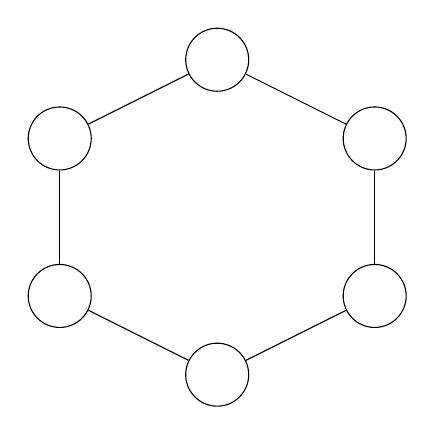
\begin{tikzpicture}
					\tikzstyle{vertex} = [circle,fill=white,draw=black]
					\tikzstyle{vertex2} = [circle,fill=white,draw=black]
					\tikzstyle{edge} = [-]
					\node[vertex,minimum size=0.8cm] (n1) at (0,0) {};
					\node[vertex2,minimum size=0.8cm] (n2) at (-2,-1) {};
					\node[vertex2,minimum size=0.8cm] (n6) at (2,-1) {};
					\node[vertex,minimum size=0.8cm] (n3) at (-2,-3) {};
					\node[vertex,minimum size=0.8cm] (n5) at (2,-3) {};
					\node[vertex2,minimum size=0.8cm] (n4) at (0,-4) {};
					\draw[edge] (n1)--(n2);
					\draw[edge] (n2)--(n3);
					\draw[edge] (n3)--(n4);
					\draw[edge] (n4)--(n5);
					\draw[edge] (n5)--(n6);
					\draw[edge] (n6)--(n1);
					\end{tikzpicture}	
				\end{center}	
				
			\end{frame}
			\begin{frame}{Upper Bound on the Span of Even Cycles }
				\begin{block}{\textit{k}-safe labeling of Even Cycles }
					Every Even Cycle with \textit{n} vertices admits a \textit{k}-safe labeling of
					\textit{n+k-1} , and such a
					labeling can be computed in linear time.
				\end{block}
				\begin{center}
					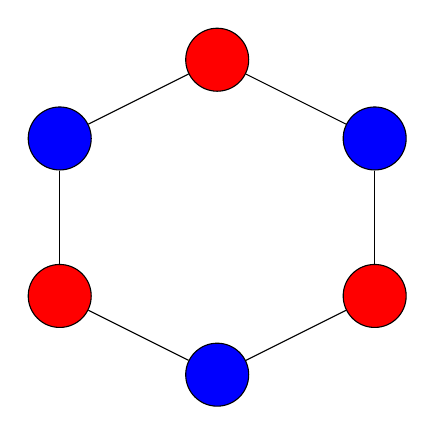
\begin{tikzpicture}
					\tikzstyle{vertex} = [circle,fill=red,draw=black]
					\tikzstyle{vertex2} = [circle,fill=blue,draw=black]
					\tikzstyle{edge} = [-]
					\node[vertex,minimum size=0.8cm] (n1) at (0,0) {};
					\node[vertex2,minimum size=0.8cm] (n2) at (-2,-1) {};
					\node[vertex2,minimum size=0.8cm] (n6) at (2,-1) {};
					\node[vertex,minimum size=0.8cm] (n3) at (-2,-3) {};
					\node[vertex,minimum size=0.8cm] (n5) at (2,-3) {};
					\node[vertex2,minimum size=0.8cm] (n4) at (0,-4) {};
					\draw[edge] (n1)--(n2);
					\draw[edge] (n2)--(n3);
					\draw[edge] (n3)--(n4);
					\draw[edge] (n4)--(n5);
					\draw[edge] (n5)--(n6);
					\draw[edge] (n6)--(n1);
					\end{tikzpicture}	
				\end{center}	
				
			\end{frame}

	\begin{frame}{Upper Bound on the Span of Odd Cycles }
		\begin{block}{\textit{k}-safe labeling of Odd Cycles }
			Every Odd Cycle with \textit{n} vertices admits a \textit{k}-safe labeling of
			\textit{n+2k-2} , and such a
			labeling can be computed in linear time.
		\end{block}
		\begin{center}
			\begin{tikzpicture}
			\tikzstyle{vertex} = [circle,fill=white,draw=black]
			\tikzstyle{vertex2} = [circle,fill=white,draw=black]
			\tikzstyle{edge} = [-]
			\node[vertex,minimum size=0.8cm] (n1) at (0,0) {};
			\node[vertex,minimum size=0.8cm] (n7) at (2,0) {};
			\node[vertex2,minimum size=0.8cm] (n2) at (-2,-1) {};
			\node[vertex2,minimum size=0.8cm] (n6) at (4,-1) {};
			\node[vertex,minimum size=0.8cm] (n3) at (-2,-3) {};
			\node[vertex,minimum size=0.8cm] (n5) at (4,-3) {};
			\node[vertex2,minimum size=0.8cm] (n4) at (1,-4) {};
			\draw[edge] (n1)--(n2);
			\draw[edge] (n2)--(n3);
			\draw[edge] (n3)--(n4);
			\draw[edge] (n4)--(n5);
			\draw[edge] (n5)--(n6);
			\draw[edge] (n1)--(n7);
			\draw[edge] (n6)--(n7);
			\end{tikzpicture}	
		\end{center}	
		
	\end{frame}
	
	\begin{frame}{Upper Bound on the Span of Odd Cycles }
		\begin{block}{\textit{k}-safe labeling of Odd Cycles }
			Every Odd Cycle with \textit{n} vertices admits a \textit{k}-safe labeling of
			\textit{n+2k-2} , and such a
			labeling can be computed in linear time.
		\end{block}
		\begin{center}
			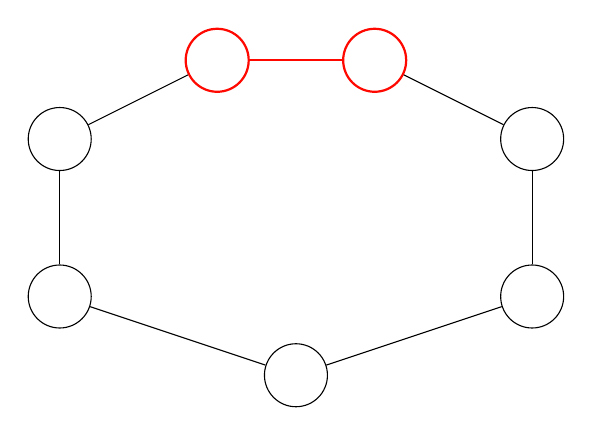
\begin{tikzpicture}
			\tikzstyle{vertex} = [circle,fill=white,draw=black]
			\tikzstyle{vertex2} = [circle,fill=white,draw=black]
			\tikzstyle{vertex3} = [circle,fill=white,draw=candyapplered,thick]
			\tikzstyle{edge} = [-]
			\tikzstyle{edge2} = [-,thick,draw = candyapplered]
			\node[vertex3,minimum size=0.8cm] (n1) at (0,0) {};
			\node[vertex3,minimum size=0.8cm] (n7) at (2,0) {};
			\node[vertex2,minimum size=0.8cm] (n2) at (-2,-1) {};
			\node[vertex2,minimum size=0.8cm] (n6) at (4,-1) {};
			\node[vertex,minimum size=0.8cm] (n3) at (-2,-3) {};
			\node[vertex,minimum size=0.8cm] (n5) at (4,-3) {};
			\node[vertex2,minimum size=0.8cm] (n4) at (1,-4) {};
			\draw[edge] (n1)--(n2);
			\draw[edge] (n2)--(n3);
			\draw[edge] (n3)--(n4);
			\draw[edge] (n4)--(n5);
			\draw[edge] (n5)--(n6);
			\draw[edge2] (n1)--(n7);
			\draw[edge] (n6)--(n7);
			\end{tikzpicture}	
		\end{center}	
		
	\end{frame}
	
		\begin{frame}{Upper Bound on the Span of Odd Cycles }
			\begin{block}{\textit{k}-safe labeling of Odd Cycles }
				Every Odd Cycle with \textit{n} vertices admits a \textit{k}-safe labeling of
				\textit{n+2k-2} , and such a
				labeling can be computed in linear time.
			\end{block}
			\begin{center}
				\begin{tikzpicture}
				\tikzstyle{vertex} = [circle,fill=white,draw=black]
				\tikzstyle{vertex2} = [circle,fill=white,draw=black]
				\tikzstyle{vertex3} = [circle,fill=white,draw=candyapplered,thick]
				\tikzstyle{edge} = [-]
				\node[vertex3,minimum size=0.8cm] (n1) at (1,0) {};
				\node[vertex2,minimum size=0.8cm] (n2) at (-2,-1) {};
				\node[vertex2,minimum size=0.8cm] (n6) at (4,-1) {};
				\node[vertex,minimum size=0.8cm] (n3) at (-2,-3) {};
				\node[vertex,minimum size=0.8cm] (n5) at (4,-3) {};
				\node[vertex2,minimum size=0.8cm] (n4) at (1,-4) {};
				\draw[edge] (n1)--(n2);
				\draw[edge] (n2)--(n3);
				\draw[edge] (n3)--(n4);
				\draw[edge] (n4)--(n5);
				\draw[edge] (n5)--(n6);
				\draw[edge] (n1)--(n6);
				\end{tikzpicture}	
			\end{center}	
			
		\end{frame}
		\begin{frame}{Upper Bound on the Span of Odd Cycles }
			\begin{block}{\textit{k}-safe labeling of Odd Cycles }
				Every Odd Cycle with \textit{n} vertices admits a \textit{k}-safe labeling of
				\textit{n+2k-2} , and such a
				labeling can be computed in linear time.
			\end{block}
			\begin{center}
				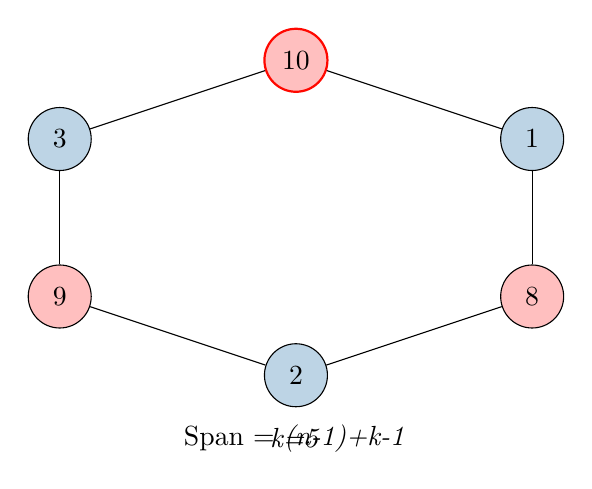
\begin{tikzpicture}
				\tikzstyle{vertex} = [circle,fill=pink,draw=black]
				\tikzstyle{vertex2} = [circle,fill=beaublue,draw=black]
				\tikzstyle{vertex3} = [circle,fill=pink,draw=candyapplered,thick]
				\tikzstyle{edge} = [-]
				\node[vertex3,minimum size=0.8cm] (n1) at (1,0) {};
				\node[vertex2,minimum size=0.8cm] (n2) at (-2,-1) {};
				\node[vertex2,minimum size=0.8cm] (n6) at (4,-1) {};
				\node[vertex,minimum size=0.8cm] (n3) at (-2,-3) {};
				\node[vertex,minimum size=0.8cm] (n5) at (4,-3) {};
				\node[vertex2,minimum size=0.8cm] (n4) at (1,-4) {};
				\draw[edge] (n1)--(n2);
				\draw[edge] (n2)--(n3);
				\draw[edge] (n3)--(n4);
				\draw[edge] (n4)--(n5);
				\draw[edge] (n5)--(n6);
				\draw[edge] (n1)--(n6);
				
				\node<7->  at (1,0) {10};
				\node<4->  at (-2,-1) {3};
				\node<2-> at (4,-1) {1};
				\node<6->  at (-2,-3) {9};
				\node<5->  at (4,-3) {8};
				\node<3->  at (1,-4) {2};
				
				\node<5-7>[] at (1,-4.8) {\textit{k=5}};
				\node<8-8>[] at (1,-4.8) {Span = \textit{(n-1)+k-1}};
				\end{tikzpicture}	
			\end{center}	
			
		\end{frame}
		
		\begin{frame}{Upper Bound on the Span of Odd Cycles }
			\begin{block}{\textit{k}-safe labeling of Odd Cycles }
				Every Odd Cycle with \textit{n} vertices admits a \textit{k}-safe labeling of
				\textit{n+2k-2} , and such a
				labeling can be computed in linear time.
			\end{block}
			\begin{center}
				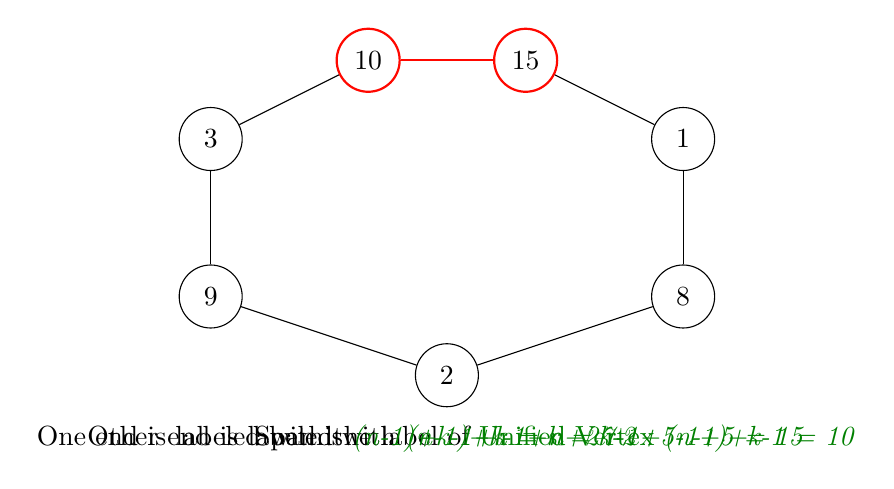
\begin{tikzpicture}
				\tikzstyle{vertex} = [circle,fill=white,draw=black]
				\tikzstyle{vertex2} = [circle,fill=white,draw=black]
				\tikzstyle{vertex3} = [circle,fill=white,draw=candyapplered,thick]
				\tikzstyle{edge} = [-]
				\tikzstyle{edge2} = [-,draw=candyapplered,thick]
				\node[vertex3,minimum size=0.8cm] (n1) at (0,0) {};
				\node[vertex3,minimum size=0.8cm] (n7) at (2,0) {};
				\node[vertex2,minimum size=0.8cm] (n2) at (-2,-1) {};
				\node[vertex2,minimum size=0.8cm] (n6) at (4,-1) {};
				\node[vertex,minimum size=0.8cm] (n3) at (-2,-3) {};
				\node[vertex,minimum size=0.8cm] (n5) at (4,-3) {};
				\node[vertex2,minimum size=0.8cm] (n4) at (1,-4) {};
				\draw[edge] (n1)--(n2);
				\draw[edge] (n2)--(n3);
				\draw[edge] (n3)--(n4);
				\draw[edge] (n4)--(n5);
				\draw[edge] (n5)--(n6);
				\draw[edge2] (n1)--(n7);
				\draw[edge] (n6)--(n7);
				
				\node  at (0,0) {10};
				\node<2->  at (2,0) {15};
				\node  at (-2,-1) {3};
				\node at (4,-1) {1};
				\node  at (-2,-3) {9};
				\node  at (4,-3) {8};
				\node  at (1,-4) {2};
				
				\node<1-1>[] at (1,-4.8) {One end is labeled with the label of \textcolor{ao(english)}{Unified Vertex \textit{(n-1)+k-1 = 10}}};
				\node<2-2>[] at (1,-4.8) {Other end is labeled with
				\textcolor{ao(english)}{\textit{(n-1)+k-1+k = 7-1+5-1+5 = 15}}};
				\node<3-3>[] at (1,-4.8) {Span is \textcolor{ao(english)}{\textit{(n-1)+k-1+k = n+2k-2}}};
				
				\end{tikzpicture}	
			\end{center}	
			
		\end{frame}
			\section{k-safe Labeling of Cactus Graphs}
			\begin{frame}
				\frametitle{Outline}
				\tableofcontents[currentsection]
			\end{frame}
			\begin{frame}{What is Biconnected Graph?}
				\centering
				\includegraphics[height=6cm,width=8cm]{bic.png}
				
				Figure : A  Biconnected Graph
			\end{frame}
			\begin{frame}{What is Biconnected Graph?}
				\centering
				\includegraphics[height=6cm,width=8cm]{bic0.png}
			\end{frame}
			\begin{frame}{What is Biconnected Graph?}
				\centering
				\includegraphics[height=6cm,width=8cm]{bic1.png}
			\end{frame}
			\begin{frame}{What is Biconnected Graph?}
				\centering
				\includegraphics[height=6cm,width=8cm]{bic2.png}
			\end{frame}
			\begin{frame}{What is Biconnected Graph?}
				\centering
				\includegraphics[height=6cm,width=8cm]{bic3.png}
			\end{frame}
			\begin{frame}{What is Biconnected Graph?}
				\centering
				\includegraphics[height=6cm,width=8cm]{bic4.png}
			\end{frame}
			\begin{frame}{What is Biconnected Graph?}
				\centering
				\includegraphics[height=6cm,width=8cm]{bic5.png}
			\end{frame}
			\begin{frame}{What is Biocnnected Component?}
				\begin{center}
					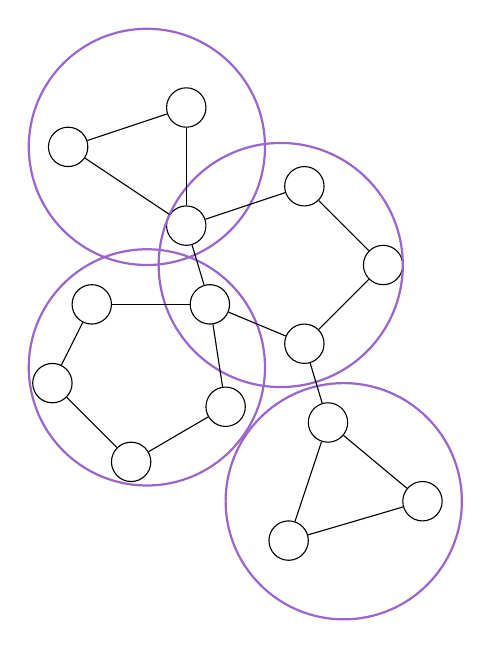
\begin{tikzpicture}
					\tikzstyle{vertex} = [circle,fill=white,draw=black]
					\tikzstyle{vertex5} = [circle,draw=amethyst,thick]
					\tikzstyle{edge} = [-]
					\node[vertex,minimum size=0.5cm] (n1) at (0,0) {};
					\node[vertex,minimum size=0.5cm] (n2) at (1.5,0.5) {};
					\node[vertex,minimum size=0.5cm] (n3) at (1.5,-1) {};
					\node[vertex,minimum size=0.5cm] (n4) at (1.8,-2) {};
					\node[vertex,minimum size=0.5cm] (n5) at (3,-2.5) {};
					\node[vertex,minimum size=0.5cm] (n6) at (4,-1.5) {};
					\node[vertex,minimum size=0.5cm] (n7) at (3,-0.5) {};
					\node[vertex,minimum size=0.5cm] (n8) at (0.3,-2) {};
					\node[vertex,minimum size=0.5cm] (n9) at (-0.2,-3) {};
					\node[vertex,minimum size=0.5cm] (n10) at (0.8,-4) {};
					\node[vertex,minimum size=0.5cm] (n11) at (2,-3.3) {};
					\node[vertex,minimum size=0.5cm] (n12) at (3.3,-3.5) {};
					\node[vertex,minimum size=0.5cm] (n13) at (2.8,-5) {};
					\node[vertex,minimum size=0.5cm] (n14) at (4.5,-4.5) {};
					\node<2-2>[vertex5,minimum size=3cm] (n17) at (1,0) {};
					\node<3-3>[vertex5,minimum size=3.1cm] (n18) at (2.7,-1.5) {};
					\node<4-4>[vertex5,minimum size=3cm] (n19) at (1,-2.8) {};
					\node<5-5>[vertex5,minimum size=3cm] (n20) at (3.5,-4.5) {};
					
					\draw[edge] (n1)--(n2);
					\draw[edge] (n2)--(n3);
					\draw[edge] (n3)--(n1);
					\draw[edge] (n3)--(n4);
					\draw[edge] (n4)--(n5);
					\draw[edge] (n5)--(n6);
					\draw[edge] (n6)--(n7);
					\draw[edge] (n7)--(n3);
					\draw[edge] (n4)--(n8);
					\draw[edge] (n8)--(n9);
					\draw[edge] (n9)--(n10);
					\draw[edge] (n10)--(n11);
					\draw[edge] (n11)--(n4);
					\draw[edge] (n5)--(n12);
					\draw[edge] (n12)--(n13);
					\draw[edge] (n13)--(n14);
					\draw[edge] (n14)--(n12);
					
					
					
					
					
					\end{tikzpicture}	
				\end{center}	
				
			\end{frame}
				\begin{frame}{What is Cactus Graph?}
					\begin{center}
						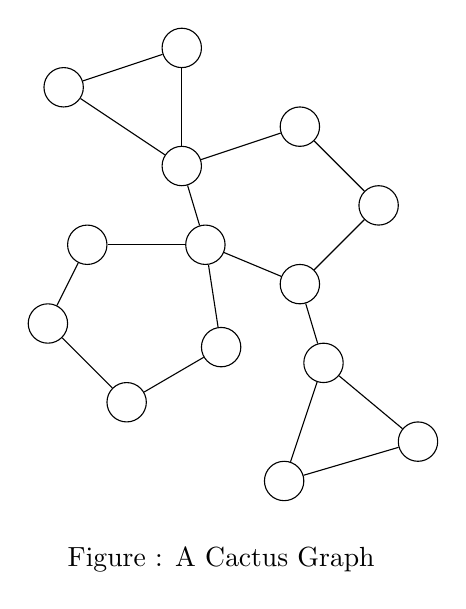
\begin{tikzpicture}
						\tikzstyle{vertex} = [circle,fill=white,draw=black]
						\tikzstyle{vertex5} = [circle,draw=amethyst,thick]
						\tikzstyle{edge} = [-]
						\node[vertex,minimum size=0.5cm] (n1) at (0,0) {};
						\node[vertex,minimum size=0.5cm] (n2) at (1.5,0.5) {};
						\node[vertex,minimum size=0.5cm] (n3) at (1.5,-1) {};
						\node[vertex,minimum size=0.5cm] (n4) at (1.8,-2) {};
						\node[vertex,minimum size=0.5cm] (n5) at (3,-2.5) {};
						\node[vertex,minimum size=0.5cm] (n6) at (4,-1.5) {};
						\node[vertex,minimum size=0.5cm] (n7) at (3,-0.5) {};
						\node[vertex,minimum size=0.5cm] (n8) at (0.3,-2) {};
						\node[vertex,minimum size=0.5cm] (n9) at (-0.2,-3) {};
						\node[vertex,minimum size=0.5cm] (n10) at (0.8,-4) {};
						\node[vertex,minimum size=0.5cm] (n11) at (2,-3.3) {};
						\node[vertex,minimum size=0.5cm] (n12) at (3.3,-3.5) {};
						\node[vertex,minimum size=0.5cm] (n13) at (2.8,-5) {};
						\node[vertex,minimum size=0.5cm] (n14) at (4.5,-4.5) {};
						\node (caption) at (2,-6) {Figure : A Cactus Graph};
						
						\draw[edge] (n1)--(n2);
						\draw[edge] (n2)--(n3);
						\draw[edge] (n3)--(n1);
						\draw[edge] (n3)--(n4);
						\draw[edge] (n4)--(n5);
						\draw[edge] (n5)--(n6);
						\draw[edge] (n6)--(n7);
						\draw[edge] (n7)--(n3);
						\draw[edge] (n4)--(n8);
						\draw[edge] (n8)--(n9);
						\draw[edge] (n9)--(n10);
						\draw[edge] (n10)--(n11);
						\draw[edge] (n11)--(n4);
						\draw[edge] (n5)--(n12);
						\draw[edge] (n12)--(n13);
						\draw[edge] (n13)--(n14);
						\draw[edge] (n14)--(n12);
						
						
						
						
						
						\end{tikzpicture}	
					\end{center}	
					
				\end{frame}
				
				\begin{frame}{Upper Bound on the Span of Cactus Graphs }
					\begin{block}{\textit{k}-safe labeling of Cactus Graphs }
						Every Cactus Graph with \textit{n} vertices admits a \textit{k}-safe labeling of
						\textit{n+2k-2} , and such a
						labeling can be computed in linear time.
					\end{block}
				\end{frame}
				
					\begin{frame}{Upper Bound on the Span of Cactus Graphs }
						\begin{block}{\textit{k}-safe labeling of Cactus Graphs }
							Every Cactus Graph with \textit{n} vertices admits a \textit{k}-safe labeling of
							\textit{n+2k-2} , and such a
							labeling can be computed in linear time.
						\end{block}
						\begin{center}
						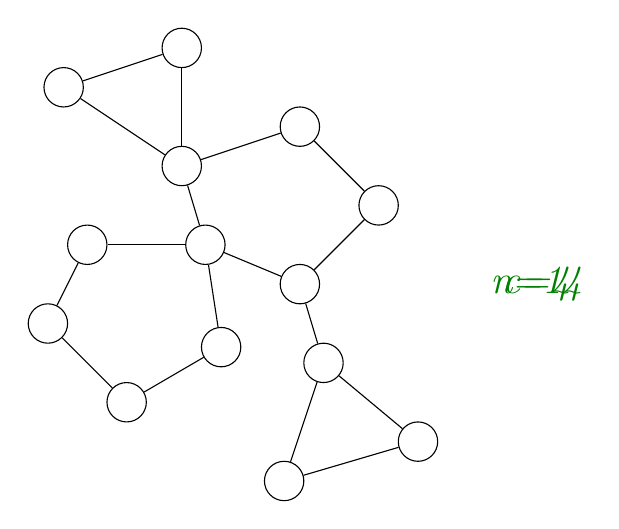
\begin{tikzpicture}
						\tikzstyle{vertex} = [circle,fill=white,draw=black]
						\tikzstyle{vertex5} = [circle,draw=amethyst,thick]
						\tikzstyle{edge} = [-]
						\node[vertex,minimum size=0.5cm] (n1) at (0,0) {};
						\node[vertex,minimum size=0.5cm] (n2) at (1.5,0.5) {};
						\node[vertex,minimum size=0.5cm] (n3) at (1.5,-1) {};
						\node[vertex,minimum size=0.5cm] (n4) at (1.8,-2) {};
						\node[vertex,minimum size=0.5cm] (n5) at (3,-2.5) {};
						\node[vertex,minimum size=0.5cm] (n6) at (4,-1.5) {};
						\node[vertex,minimum size=0.5cm] (n7) at (3,-0.5) {};
						\node[vertex,minimum size=0.5cm] (n8) at (0.3,-2) {};
						\node[vertex,minimum size=0.5cm] (n9) at (-0.2,-3) {};
						\node[vertex,minimum size=0.5cm] (n10) at (0.8,-4) {};
						\node[vertex,minimum size=0.5cm] (n11) at (2,-3.3) {};
						\node[vertex,minimum size=0.5cm] (n12) at (3.3,-3.5) {};
						\node[vertex,minimum size=0.5cm] (n13) at (2.8,-5) {};
						\node[vertex,minimum size=0.5cm] (n14) at (4.5,-4.5) {};
						\node<1-1> (c0) at (6,-2.5) {\textit{\Large{\textcolor{ao(english)}{n=14}}}};
						\node<2-2> (c1) at (6,-2.5) {\textit{\Large{\textcolor{ao(english)}{c=4}}}};
						
						\draw[edge] (n1)--(n2);
						\draw[edge] (n2)--(n3);
						\draw[edge] (n3)--(n1);
						\draw[edge] (n3)--(n4);
						\draw[edge] (n4)--(n5);
						\draw[edge] (n5)--(n6);
						\draw[edge] (n6)--(n7);
						\draw[edge] (n7)--(n3);
						\draw[edge] (n4)--(n8);
						\draw[edge] (n8)--(n9);
						\draw[edge] (n9)--(n10);
						\draw[edge] (n10)--(n11);
						\draw[edge] (n11)--(n4);
						\draw[edge] (n5)--(n12);
						\draw[edge] (n12)--(n13);
						\draw[edge] (n13)--(n14);
						\draw[edge] (n14)--(n12);
						\end{tikzpicture}	
					\end{center}
					\end{frame}
					
					\begin{frame}{Upper Bound on the Span of Cactus Graphs }
						\begin{block}{\textit{k}-safe labeling of Cactus Graphs }
							Every Cactus Graph with \textit{n} vertices admits a \textit{k}-safe labeling of
							\textit{n+2k-2} , and such a
							labeling can be computed in linear time.
						\end{block}
						\begin{center}
							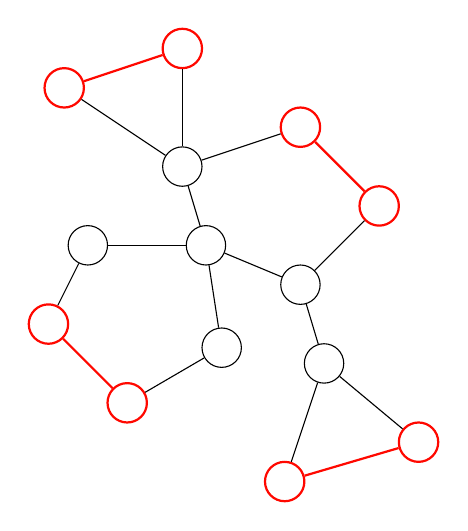
\begin{tikzpicture}
							\tikzstyle{vertex} = [circle,fill=white,draw=black]
							\tikzstyle{vertex2} = [circle,fill=white,draw=candyapplered,thick]
							//\tikzstyle{vertex3} = [circle,fill=white,draw=candyapplered,thick]
							\tikzstyle{edge} = [-]
							\tikzstyle{edge2} = [-,draw=candyapplered,thick]
							\node[vertex2,minimum size=0.5cm] (n1) at (0,0) {};
							\node[vertex2,minimum size=0.5cm] (n2) at (1.5,0.5) {};
							\node[vertex,minimum size=0.5cm] (n3) at (1.5,-1) {};
							\node[vertex,minimum size=0.5cm] (n4) at (1.8,-2) {};
							\node[vertex,minimum size=0.5cm] (n5) at (3,-2.5) {};
							\node[vertex2,minimum size=0.5cm] (n6) at (4,-1.5) {};
							\node[vertex2,minimum size=0.5cm] (n7) at (3,-0.5) {};
							\node[vertex,minimum size=0.5cm] (n8) at (0.3,-2) {};
							\node[vertex2,minimum size=0.5cm] (n9) at (-0.2,-3) {};
							\node[vertex2,minimum size=0.5cm] (n10) at (0.8,-4) {};
							\node[vertex,minimum size=0.5cm] (n11) at (2,-3.3) {};
							\node[vertex,minimum size=0.5cm] (n12) at (3.3,-3.5) {};
							\node[vertex2,minimum size=0.5cm] (n13) at (2.8,-5) {};
							\node[vertex2,minimum size=0.5cm] (n14) at (4.5,-4.5) {};
							
							\draw[edge2] (n1)--(n2);
							\draw[edge] (n2)--(n3);
							\draw[edge] (n3)--(n1);
							\draw[edge] (n3)--(n4);
							\draw[edge] (n4)--(n5);
							\draw[edge] (n5)--(n6);
							\draw[edge2] (n6)--(n7);
							\draw[edge] (n7)--(n3);
							\draw[edge] (n4)--(n8);
							\draw[edge] (n8)--(n9);
							\draw[edge2] (n9)--(n10);
							\draw[edge] (n10)--(n11);
							\draw[edge] (n11)--(n4);
							\draw[edge] (n5)--(n12);
							\draw[edge] (n12)--(n13);
							\draw[edge2] (n13)--(n14);
							\draw[edge] (n14)--(n12);
							\end{tikzpicture}	
						\end{center}	
						
					\end{frame}
					
						\begin{frame}{Upper Bound on the Span of Cactus Graphs }
							\begin{block}{\textit{k}-safe labeling of Cactus Graphs }
								Every Cactus Graph with \textit{n} vertices admits a \textit{k}-safe labeling of
								\textit{n+2k-2} , and such a
								labeling can be computed in linear time.
							\end{block}
							\begin{center}
								\begin{tikzpicture}
							\tikzstyle{vertex} = [circle,fill=white,draw=black]
							\tikzstyle{vertex2} = [circle,fill=white,draw=candyapplered,thick]
							//\tikzstyle{vertex3} = [circle,fill=white,draw=candyapplered,thick]
							\tikzstyle{edge} = [-]
							\tikzstyle{edge2} = [-,draw=candyapplered,thick]
							\node[vertex2,minimum size=0.5cm] (n1) at (0,0) {};
							\node[vertex,minimum size=0.5cm] (n3) at (1.5,-1) {};
							\node[vertex,minimum size=0.5cm] (n4) at (1.8,-2) {};%
							\node[vertex,minimum size=0.5cm] (n5) at (3,-2.5) {};
							%\node[vertex,minimum size=0.5cm] (n6) at (4,-1.5) {};
							%/\node[vertex2,minimum size=0.5cm] (n7) at (3,-0.5) {};
							\node[vertex2,minimum size=0.5cm] (n15) at (3,-1.3) {};%
							\node[vertex,minimum size=0.5cm] (n8) at (0.3,-2) {};
							%\node[vertex2,minimum size=0.5cm] (n9) at (-0.2,-3) {};
							%\node[vertex2,minimum size=0.5cm] (n10) at (0.8,-4) {};
							\node[vertex2,minimum size=0.5cm] (n16) at (0.3,-3.5) {};%
							\node[vertex,minimum size=0.5cm] (n11) at (2,-3.3) {};
							\node[vertex,minimum size=0.5cm] (n12) at (3.3,-3.5) {};%
							\node[vertex2,minimum size=0.5cm] (n13) at (2.8,-5) {};
							%\node[vertex2,minimum size=0.5cm] (n14) at (4.5,-4.5) {};
							
							%\draw[edge2] (n1)--(n2);
							%\draw[edge] (n2)--(n3);
							\draw[edge] (n3)--(n1);
							\draw[edge] (n3)--(n4);
							\draw[edge] (n4)--(n5);
							\draw[edge] (n5)--(n15);
							%\draw[edge] (n6)--(n15);
							\draw[edge] (n15)--(n3);
							\draw[edge] (n4)--(n8);
							\draw[edge] (n8)--(n16);
							%\draw[edge2] (n9)--(n10);
							\draw[edge] (n16)--(n11);
							\draw[edge] (n11)--(n4);
							\draw[edge] (n5)--(n12);
							\draw[edge] (n12)--(n13);
							\node (c0) at (6,-2.5) {\Large{{\textit{\textcolor{ao(english)}{n-c}}} vertices}};
								\end{tikzpicture}	
							\end{center}	
							
						\end{frame}
						
							\begin{frame}{Upper Bound on the Span of Cactus Graphs }
								\begin{block}{\textit{k}-safe labeling of Cactus Graphs }
									Every Cactus Graph with \textit{n} vertices admits a \textit{k}-safe labeling of
									\textit{n+2k-2} , and such a
									labeling can be computed in linear time.
								\end{block}
								\begin{center}
									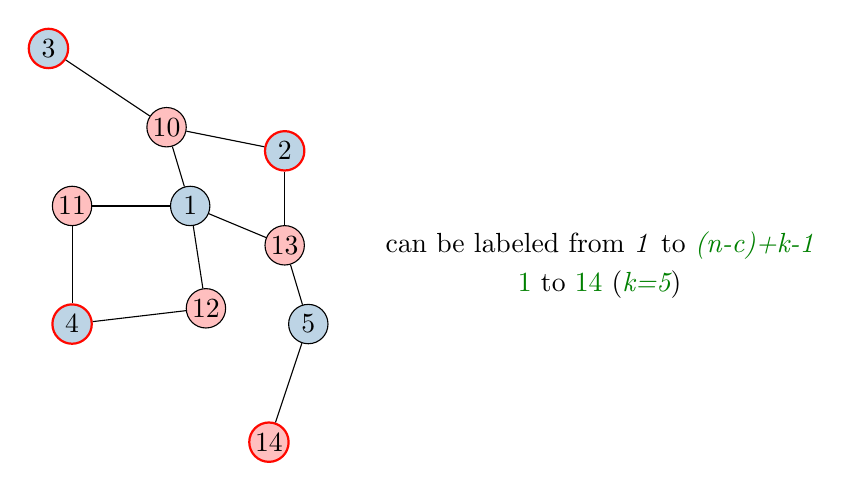
\begin{tikzpicture}
								\tikzstyle{vertex} = [circle,fill=pink,draw=black]
								\tikzstyle{vertex2} = [circle,fill=beaublue,draw=candyapplered,thick]
								\tikzstyle{vertex3} = [circle,fill=beaublue,draw=black]
								\tikzstyle{vertex4} = [circle,fill=pink,draw=candyapplered,thick]
								
								\tikzstyle{edge} = [-]
								\tikzstyle{edge2} = [-,draw=candyapplered,thick]
								\node[vertex2,minimum size=0.5cm] (n1) at (0,0) {}; %
								%\node[vertex2,minimum size=0.5cm] (n2) at (1.5,0.5) {};
								\node[vertex,minimum size=0.5cm] (n3) at (1.5,-1) {};
								\node[vertex3,minimum size=0.5cm] (n4) at (1.8,-2) {};%
								\node[vertex,minimum size=0.5cm] (n5) at (3,-2.5) {};
								%\node[vertex,minimum size=0.5cm] (n6) at (4,-1.5) {};
								%/\node[vertex2,minimum size=0.5cm] (n7) at (3,-0.5) {};
								\node[vertex2,minimum size=0.5cm] (n15) at (3,-1.3) {};%
								\node[vertex,minimum size=0.5cm] (n8) at (0.3,-2) {};
								%\node[vertex2,minimum size=0.5cm] (n9) at (-0.2,-3) {};
								%\node[vertex2,minimum size=0.5cm] (n10) at (0.8,-4) {};
								\node[vertex2,minimum size=0.5cm] (n16) at (0.3,-3.5) {};%
								\node[vertex,minimum size=0.5cm] (n11) at (2,-3.3) {};
								\node[vertex3,minimum size=0.5cm] (n12) at (3.3,-3.5) {};%
								\node[vertex4,minimum size=0.5cm] (n13) at (2.8,-5) {};
								%\node[vertex2,minimum size=0.5cm] (n14) at (4.5,-4.5) {};
								
								
								%\draw[edge2] (n1)--(n2);
								%\draw[edge] (n2)--(n3);
								\draw[edge] (n3)--(n1);
								\draw[edge] (n3)--(n4);
								\draw[edge] (n4)--(n5);
								\draw[edge] (n5)--(n15);
								%\draw[edge] (n6)--(n15);
								\draw[edge] (n15)--(n3);
								\draw[edge] (n4)--(n8);
								\draw[edge] (n8)--(n16);
								%\draw[edge2] (n9)--(n10);
								\draw[edge] (n16)--(n11);
								\draw[edge] (n11)--(n4);
								\draw[edge] (n5)--(n12);
								\draw[edge] (n12)--(n13);
								%\draw[edge2] (n13)--(n14);
								%\draw[edge] (n14)--(n12);
								
								
								%labels				
								\node<4->  at (0,0) {3};
								\node<7->  at (1.5,-1) {10};
								\node<3->  at (3,-1.3) {2};
								\node<2-> at (1.8,-2) {1};
								\node<10->  at (3,-2.5) {13};
								\node<6->  at (3.3,-3.5) {5};
								\node<11->  at (2.8,-5) {14};
								\node<8-> at (0.3,-2) {11};
								\node<5-> at (0.3,-3.5) {4};
								\node<9-> at (2,-3.3) {12};
								
								\node<1-1> (c0) at (7,-2.5) {can be labeled from \textit{1} to {\textit{\textcolor{ao(english)}{(n-c)+k-1}}}};
								\node<1-1> (c1) at (7,-3) {\textcolor{ao(english)}{1} to \textcolor{ao(english)}{14}  (\textit{\textcolor{ao(english)}{k=5}}) };
									\end{tikzpicture}	
								\end{center}	
								
							\end{frame}
							
								\begin{frame}{Upper Bound on the Span of Cactus Graphs }
									\begin{block}{\textit{k}-safe labeling of Cactus Graphs }
										Every Cactus Graph with \textit{n} vertices admits a \textit{k}-safe labeling of
										\textit{n+2k-2} , and such a
										labeling can be computed in linear time.
									\end{block}
									\begin{center}
										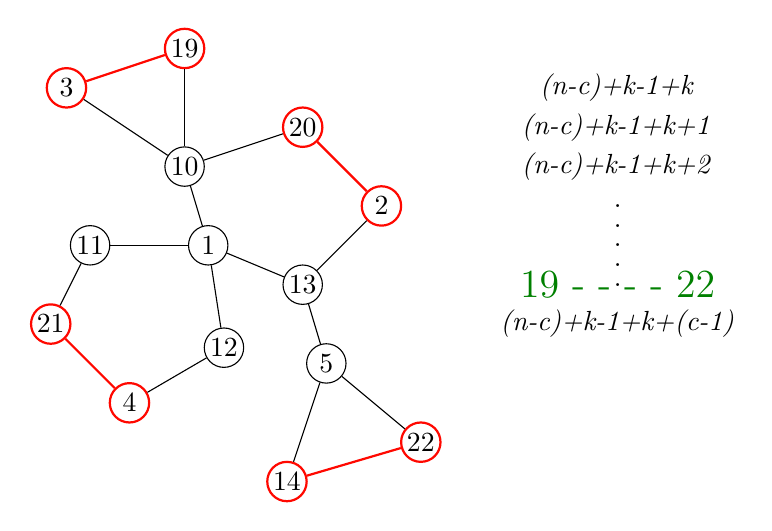
\begin{tikzpicture}
										\tikzstyle{vertex} = [circle,fill=white,draw=black]
										\tikzstyle{vertex2} = [circle,fill=white,draw=candyapplered,thick]
										//\tikzstyle{vertex3} = [circle,fill=white,draw=candyapplered,thick]
										\tikzstyle{edge} = [-]
										\tikzstyle{edge2} = [-,draw=candyapplered,thick]
										\node[vertex2,minimum size=0.5cm] (n1) at (0,0) {};
										\node[vertex2,minimum size=0.5cm] (n2) at (1.5,0.5) {};
										\node[vertex,minimum size=0.5cm] (n3) at (1.5,-1) {};
										\node[vertex,minimum size=0.5cm] (n4) at (1.8,-2) {};
										\node[vertex,minimum size=0.5cm] (n5) at (3,-2.5) {};
										\node[vertex2,minimum size=0.5cm] (n6) at (4,-1.5) {};
										\node[vertex2,minimum size=0.5cm] (n7) at (3,-0.5) {};
										\node[vertex,minimum size=0.5cm] (n8) at (0.3,-2) {};
										\node[vertex2,minimum size=0.5cm] (n9) at (-0.2,-3) {};
										\node[vertex2,minimum size=0.5cm] (n10) at (0.8,-4) {};
										\node[vertex,minimum size=0.5cm] (n11) at (2,-3.3) {};
										\node[vertex,minimum size=0.5cm] (n12) at (3.3,-3.5) {};
										\node[vertex2,minimum size=0.5cm] (n13) at (2.8,-5) {};
										\node[vertex2,minimum size=0.5cm] (n14) at (4.5,-4.5) {};
										
										\draw[edge2] (n1)--(n2);
										\draw[edge] (n2)--(n3);
										\draw[edge] (n3)--(n1);
										\draw[edge] (n3)--(n4);
										\draw[edge] (n4)--(n5);
										\draw[edge] (n5)--(n6);
										\draw[edge2] (n6)--(n7);
										\draw[edge] (n7)--(n3);
										\draw[edge] (n4)--(n8);
										\draw[edge] (n8)--(n9);
										\draw[edge2] (n9)--(n10);
										\draw[edge] (n10)--(n11);
										\draw[edge] (n11)--(n4);
										\draw[edge] (n5)--(n12);
										\draw[edge] (n12)--(n13);
										\draw[edge2] (n13)--(n14);
										\draw[edge] (n14)--(n12);
										
										\node at (0,0) {3};%
										\node at (1.5,-1) {10};%
										\node  at (4,-1.5) {2};%
										\node at (1.8,-2) {1};%
										\node  at (3,-2.5) {13};%
										\node  at (3.3,-3.5) {5};%
										\node  at (2.8,-5) {14};%
										\node at (0.3,-2) {11};%
										\node at (0.8,-4) {4};
										\node at (2,-3.3) {12};%
										\node<4-> at (1.5,0.5) {19};%
										\node<5-> at (3,-0.5) {20};%
										\node<7-> at (4.5,-4.5) {22};%
										\node<6-> at (-0.2,-3) {21};%
										
										\node<2-2> (c0) at (7,0) {\textit{(n-c)+k-1+k}};
										\node<2-2> (c1) at (7,-0.5) {\textit{(n-c)+k-1+k+1}};
										\node<2-2> (c2) at (7,-1) {\textit{(n-c)+k-1+k+2}};
										\node<2-2> (c3) at (7,-1.5) {.};
										\node<2-2> (c8) at (7,-1.75) {.};
										\node<2-2> (c7) at (7,-2.25) {.};
										\node<2-2> (c4) at (7,-2) {.};
										\node<2-2> (c5) at (7,-2.5) {.};
										\node<2-2> (c6) at (7,-3) {\textit{(n-c)+k-1+k+(c-1)}};
										\node <3-3>(c) at (7,-2.5) {\Large{{\textcolor{ao(english)}{19 - - - - 22}}}};
										\end{tikzpicture}	
									\end{center}	
									
								\end{frame}
								\begin{frame}{Upper Bound on the Span of Cactus Graphs }
									\begin{block}{\textit{k}-safe labeling of Cactus Graphs }
										Every Cactus Graph with \textit{n} vertices admits a \textit{k}-safe labeling of
										\textit{n+2k-2} , and such a
										labeling can be computed in linear time.
									\end{block}
									\begin{itemize}
										\item[]
										\item[]
										\item[$\bigstar$] \Large{ Span is \textcolor{ao(english)}{n-c+k-1+k+c-1} = \textcolor{ao(english)}{n+2k-2}}
									\end{itemize}
									
								\end{frame}
								
			\section{Conclusion}
			\begin{frame}
				\frametitle{Outline}
				\tableofcontents[currentsection]
			\end{frame}
			\begin{frame}{Future Interests}
				\begin{itemize}
						\item<1->[\Large{$\bigstar$}] \Large{Finding non-trivial bounds for general graphs and other subclasses of graphs.}
						\item<2->[$\bigstar$] \Large{Finding more tight upper bounds for Trees and Cactus graphs}
						\item<3->[$\bigstar$] \Large{Proving NP-hardness for subclasses of graphs}
						
				\end{itemize}
			\end{frame}
			\begin{frame}
				\begin{center}
				\vskip20pt
				\begin{tikzpicture}
				\node at (0,0) {\Huge{\Huge{Thank You !!!}}};
				\node at (3.5,0) {\includegraphics[height=1cm,width=1cm]{smily.png}};
				\end{tikzpicture}
			\end{center}
				
			\end{frame}
		
		
		
	

\end{document}
